\documentclass[11 pt]{article}
\usepackage{graphicx}
\usepackage[export]{adjustbox}
\usepackage{float}
\usepackage{amsmath}
\usepackage{pgfplots}
\pgfplotsset{compat=1.15}
\title{EE362 Induction Machine}
\date{2018\\ April}
\author{Nail Tosun - 2094563 \\ Electric and Electronic Engineering Departmant, METU}
\begin{document}
\maketitle
\section*{Induction Motor Tests}
\subsection*{No-load test}
It is the same as open circuit test of transformer. It gives information about \textbf{\textit{rotational loss}} and \textbf{\textit{excitation current}}.

Since there is no load;
$$s=0$$
Then equivalent circuit becomes;
\begin{figure}[H]
\centering
  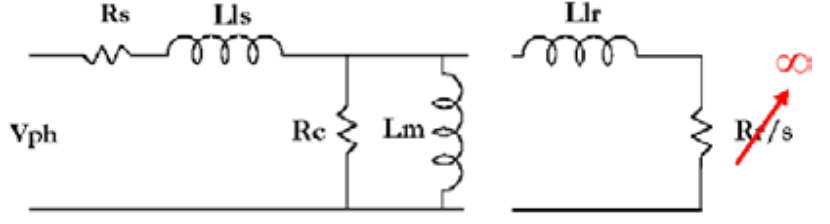
\includegraphics[scale=0.6]{no-load}
  \caption{No-load equivalent circuit}
  \label{fig:zero}
\end{figure}
The values we obtain from no load test are;
\begin{table}[]
\centering
\caption{test result}
\label{my-label}
\begin{tabular}{lcccl}
$V_{line to line}$    & $I_0$ & $I_{max}$ & P  & $f_s$ \\
208 V & 1.5A  & 1.7 A   & 49 & 60 Hz
\end{tabular}
\end{table}
\[V_{ph}=\frac{208}{\sqrt{3}}=121.1 V\]
\[cos(\phi)=\frac{\frac{P_{3\phi}}{3}}{V_{ph} I_{Ph}}=0.09\]
\[\phi=84.8\deg\]
\[I_m=I_0 sin(\phi)=1.485 A\]
\[I_c=I_0 cos(\phi)=0.135 A\]
Now assuming $R_c$ is much greater than $R_s$;
\[L_m=X_m=\frac{V_{ph}}{2\pi f_sI_m}\]
\[L_m=0.23H\]
\[R_c=\frac{V_{ph}}{I_c}\]
\[R_c=900 ohm\]
\subsection*{Locked rotor test}
Since rotor is stationary with mechanical brake, $f_r=0$ and 
$$s=1$$
\begin{figure}[H]
\centering
  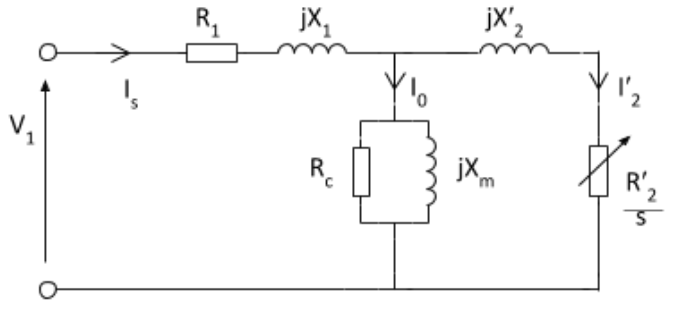
\includegraphics[scale=0.6]{locked}
  \caption{Locked-rotor test equivalent circuit}
  \label{fig:zero}
\end{figure}
Find $R_1$ with dc resistance test. How?
\subsubsection*{DC resistance test}
If machine is Y-connected, put dc supply (low voltage reference to its rated) measure the current.
\[2R_Y=\frac{V_{in}}{I_{measured}}\]
\[R_Y=\frac{1}{2}\frac{V_{in}}{I_{measured}}\]
\begin{figure}[H]
\centering
  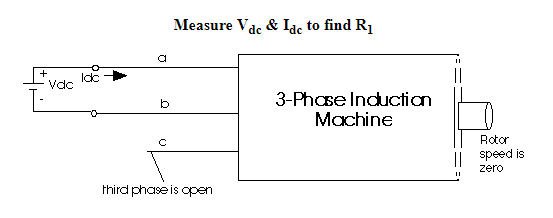
\includegraphics[scale=0.7]{dcy}
  \caption{Testing dc resistance for Y-connected ac machine}
  \label{fig:zero}
\end{figure}
If ac machine delta connected,
\[\frac{V_{in}}{I_{measured}}=R_d || 2R_d\]
\[R_d=\frac{3}{2}\frac{V_{in}}{I_{measured}}\]
Now ac resistance of $R_1$ is approximately $R_{1_{ac}}=1.1 R_{1_{dc}}$
\[V_{ph}=I\]
\subsection*{Example}
For an induction motor following test results are obtained;
\begin{table}[H]
\centering
\caption{Test results}
\label{my-label}
\begin{tabular}{lccc}
                  & Line voltage & Line current & Input power \\
Locked rotor test & 130 V        & 77 A         & 6.4 kW      \\
No-load test      & 415 V        & 22.8 V       & 1.65 kW    
\end{tabular}
\end{table}
Machine rating; 30kW 3-ph, 50 Hz, 4-pole, 415 V, delta-connected
\[r_{1_dc}=0.44\>\>ohm\]
Assume $X_1=X_2$
\subsubsection*{Solution}
\[r_{1_ac}=1.1r_{1_dc}=0.48 \> ohm\]
\end{document}